\documentclass{scrartcl}
\usepackage[ngerman]{babel}
\usepackage[utf8]{inputenc}
\usepackage{amsmath}
\usepackage{graphicx}
\usepackage{tabularx}
\usepackage{amssymb}
\usepackage{hyperref}
\usepackage{enumitem}
%\renewcommand{\contentsname}{Inhaltsverzeichnis}
\begin{document}
\title{
    \hspace{-0.5cm} 
\includegraphics[height=5cm]{resources/logo.png} \\[1cm]
    \Huge{YUV.KA} \\ \large{Praxis der Softwareentwicklung 2011/2012}
}
\author{Max Wagner $\cdot$ Patrick Gemander $\cdot$ Sebastian Ullrich $\cdot$ Michael Vollmer \\ Robert Hangu $\cdot$ Daniel Lebert}
\maketitle

\newpage
\mbox{}
\newpage
\mbox{}

\addcontentsline{toc}{section}{Inhaltsverzeichnis}
\tableofcontents
\section{Einleitung}

Es soll ein Multimedia-Framework zur Evaluation von Videoencodern erstellt werden. Hierzu werden unkomprimierte Videos eingelesen, welche anschließend mit verschiedenen Syntheseoptionen verändert werden können. Anschließend sollen die manipulierten Videos von einem externen Videoencoder, der mit dem H.264 Codec arbeitet, encodiert werden. Die so erzeugten und veränderten Videos sollen außerdem mit Referenzvideos verglichen werden, um eventuelle Schwächen des Encoders aufzuzeigen. Dieser Vergleich soll durch diverse Anzeigeoptionen dargestellt werden. In diese Analyse sollen auch die durch die Encodierung anfallenden Informationen des Encoders einfließen.

\section{Zielbestimmung}

Der Benutzer soll durch das Produkt in die Lage versetzt werden, Videoencoder zu testen, indem Videos manipuliert, encodiert und anhand eines Referenzvideos verglichen werden.

\subsection{Musskriterien}

\begin{itemize}
	\item Eingabe von unkomprimierten Videos, einer festen Farbe, einem Bild oder Noise.
	\item Manipulation der Videos
	\begin{itemize}
		\item Erstellen einer Pipeline mit verschiedenen Manipulationsoptionen.
		\item Zusammenstellung über knotenbasierte GraphView
	\end{itemize}
	\item Analyse der Videos
	\begin{itemize}
		\item Anzeigen verschiedener Diagramme.
		\item Videoausgabe mit optionalen Overlayoptionen.
	\end{itemize}
	\item Speichern von Videos und Pipeline.
\end{itemize}

\subsection{Wunschkriterien}

\begin{itemize}
	\item Benutzern eine Undo/Redo-Funktion bieten.
	\item Verwenden von Tabs im Interface.
	\item Benutzern die Möglichkeit bieten, die Aufösung der eingegebenen Videos automatisch zu erkennen.
	\item Verwenden einer asynchronen, nichtblockenden UI.
	\item Ausnutzen von Multithreading-Möglichkeiten.
	\item Verarbeiten der Motionvektoren des Encoders.
	\item Erweiterbarkeit der Knotenmenge durch Plugins.
\end{itemize}

\subsection{Abgrenzungskriterien}

\begin{itemize}
	\item Keine Soundausgabe
	\item Nur YUV-Videos als Eingabe zugelassen
    \item Keine Unterstützung für Bildtransparenz
	\item Keine Speicherung der Analysedaten
\end{itemize}

\section{Produkteinsatz}

Das Produkt dient zum Testen der eigens entwickelten Encoder bzw. deren Videos.

\subsection{Anwendungsbereiche}

Manipulation und Analyse von Videos (professioneller Anwendungsbereich)

\subsection{Zielgruppen}

Die Zielgruppe sind Entwickler des zu testenden Encoders, sodass ein gewisses Vorwissen über Videomanipulation vorrausgesetzt werden kann.

\subsection{Betriebsbedingungen}

Einsatz in der Entwurfsumgebung, in der auch die Encoder entwickelt wurden.

\section{Produktumgebung}

\begin{description}[style=multiline,leftmargin=3.5cm]
	\item[Betriebssystem] Windows 7
	\item[.NET Framework] 4.0
	\item[Prozessor] 2 GHz Taktfrequenz oder schneller
	\item[Hauptspeicher] 2 GB oder mehr
	\item[Graphikkarte] DirectX-9-kompatibel
\end{description}

\section{Funktionale Anforderungen}

\subsection{Input/Output zur Videobearbeitung}
 
\begin{description}
        \item[/F10/]YUV-Dateien einlesen \label{F10}\newline
                Als YUV-Datei gespeicherte Videos sollen eingelesen und anschließend bearbeitet werden können.
        \item[/F20/]PNG-Dateien als Standbildvideo \label{F20}\newline
                PNG-Dateien sollen eingelesen und als Standbild abgespielt werden können. Der Benutzer erhält hiermit ein Video, das nur das eingelesene Standbild zeigt.
        \item[/F30/]Standbildbibliothek \newline
                Der Benutzer soll in der Lage sein auf einfache Weise einen Standbildinput abzurufen. Vorgegebene Standbilder werden beispielsweise ein komplett rotes Bild sein.
        \item[/F40/]Perlin-Noise \newline
                Der Benutzer soll Perlin-Noise als Videoinput erzeugen können.
        \item[/F50/]Speichern von YUV-Dateien \newline
                Eventuell veränderte Videos sollen im YUV-Format gespeichert werden können.
        \item[/F60/]Speichern von Pipelines \label{F60}\newline
                Das Programm soll die erstellten Bearbeitungs- und Analysepipelines speichern und laden können.
        \item[/F70/]Anzeigen von (bearbeiteten) Videos
\end{description}
 
\subsection{Videobearbeitung}
\begin{description}
        \item[/F100/]RGB-Trennung \newline
                 Der Benutzer soll ein Video so auftrennen können, dass er drei Videos erhält, von denen das Erste nur den roten Anteil, das Zweite nur den grünen Anteil und das Dritte nur den blauen Anteil des aufgetrennten Videos zeigt.
        \item[/F110/]Additives Übereinanderlegen von Videos \newline
                Mehrere Videos sollen durch Addition ihrer Pixelwerte übereinandergelegt werden können. Hierbei werden die Farbwerte der positionsgleichen Pixel der Videos aufaddiert und als neuer Farbwert des entstehenden Videos interpretiert.
        \item[/F120/]Gewichtet gemitteltes Übereinanderlegen von  Videos \newline
                Der Benutzer soll in der Lage sein mehrere Videos gemittelt übereinander zu legen. Hierbei werden die Farbwerte positionsgleicher Pixel gewichtet aufaddiert und anschließend gemittelt, um im gegebenen Farbbereich zu bleiben. Der Benutzer ist außerdem in der Lage die Gewichtung selbst festzulegen.
        \item[/F130/]Lineares und Gauß'sches Weichzeichnen \newline
                Lineares und Gauß'sches Weichzeichnen von Videos soll möglich sein.
        \item[/F140/]Farbinvertierung \newline
                Eine Farbinvertierung der Videos soll möglich sein.
        \item[/F150/]Kontrast, Farbsättigung und Helligkeit editieren \newline
                Der Benutzer soll in der Lage sein den Kontrast, die Farbsättigung und die Helligkeit der Videos zu verändern.
        \item[/F160/]Verzögern eines Videos um $n$ Frames \newline
                Der Benutzer soll ein Video um $n$ Frames nach hinten versetzen.       
        \item[/F170/]Bilden des Differenzvideos zweier Videos \newline
                Es soll möglich sein das Differenzvideo durch Subtraktion der Farbwerte positionsgleicher Pixel der beiden Videos zu erstellen.
	\item[/F180/]Verwendung eines Videoencoders \newline
		Der Benutzer soll in der Lage sein den zu testenden Videoencoder in die Pipeline einzubauen.
\end{description}
 
\subsection{Videoanalyse}
\subparagraph{Analyse eines einzelnen Videos} 
	\begin{description}
	        \item[/F200/]Anzeigen des Inter/Intra-Block/Verhältnisses pro Frame
                \item[/F210/]Anzeigen des Helligkeitsverlaufs eines Videos pro Frame
                \item[/F220/]Anzeigen des Histogramms eines Video
                \item[/F230/]Anzeigen der peak signal-to-noise ratio pro Frame
        \end{description}
\subparagraph{Vergleich eines oder mehrerer Videos mit einem Referenzvideo}
        \begin{description}
   	        \item[/F300/]Anzeigen der Differenzen der Pixelfarben
                \item[/F310/]Anzeigen der Differenz der Encoder-Entscheidungen pro Frame
                \item[/F320/]Anzeigen der Anzahl der Artefakte pro Frame
                \item[/F330/]Videoansicht mit Artefakthighlighting \newline
			Der Benutzer soll sich eine Ansicht anzeigen lassen können, die ihm die Artefakte im Bezug auf das Referenzvideo hervorhebt.
        \end{description}  
\subsection{Sonstiges}
	\begin{description}
		\item[/F400/]Im Video springen \newline
			Der Benutzer soll sowohl bei laufendem, als auch bei nicht laufendem Video an einen beliebigen Punkt im Video springen können.
		\item[/F410/]Video schneller/langsamer abspielen \newline
			Der Benutzer soll in der Lage sein das Video auf doppelter und halber Geschwindigkeit abzuspielen.	
  		\item[/F410/]Kombinierbarkeit \newline
			Die Punkte /F10/ bis /F330/ sollen im Rahmen der Rechnerleistung beliebig kombinierbar sein.
        \end{description}

\subsection{Wunschkriterien}
	\begin{description}
		\item[/F500/]Plugins \newline
			Das Programm soll durch Plugins um weitere Knotentypen erweiterbar sein.
		\item[/F510/]Quantisieren der Farbpalette eines Videos \newline
			Die Farbpalette eines Videos soll quantisiert werden können.
	\end{description}

 


\section{Nichtfunktionale Anforderungen}

\subparagraph{Benutzbarkeit}
\begin{description}
	\item[/NF10/] Die Benutzeroberfläche soll einfach und intuitiv zu bedienen sein. Unerfahrene Benutzer sollen ohne Vorwissen in der Lage sein, sich schnell in die Funktionalitäten einzuarbeiten.
	\item[/NF20/] Die Zusammenstellung sowie die Nacheinanderreihung der verschiedenen Manipulationseffekte soll einfach und übersichtlich geschehen können. 
	\item[/NF30/] Der Benutzer muss in der Lage sein, neue Manipulationseffekte hinzuzufügen, ohne die Reihenfolge der bereits bestehenden ändern zu müssen.
	\item[/NF40/] Im Programm sollen theoretisch gleichzeitig uneingeschränkt viele Videos verwaltet, bearbeitet und analysiert werden können.
	\item[/NF50/] Der Benutzer muss ein Video aus jeder Stufe der Bearbeitung problemlos abspielen, analysieren oder exportieren können.
\end{description}

\subparagraph{Geschwindigkeit}

\begin{description}
	\item[/NF100/] Bei einer einfachen analysefähigen Pipeline mit einem einzigen Manipulationseffekt sollen ein Video der Auflösung 320p und die zugehörigen Statistiken in angemessener Geschwindigkeit
 ausgegeben werden können.
\end{description}

\subparagraph{Robustheit}

\begin{description}
	\item[/NF200/] Das Programm soll trotz falscher Benutzereingaben oder Parameter nicht abstürzen. Es muss in diesen Fällen entsprechend reagieren.
\end{description}

\subparagraph{Erweiterbarkeit}

\begin{description}
	\item[/NF300/] Das Programm soll sich einfach um neue Funktionalitäten erweitern lassen.
\end{description}

\section{Produktdaten}
\label{sec:produktdaten}

\begin{description}
	\item[/PD10/] Videodateien \\
        Es können Dateien im IYUV-Format\footnote{\url{http://www.fourcc.org/yuv.php\#IYUV}} eingelesen und ausgegeben werden; zusätzlich kann der Encoder eine Logdatei bereitstellen, in der pro Macroblock des zugehörigen Videos die Inter/Intra-Frame-Entscheidung und der Move Vector dokumentiert sind.
	\item[/PD20/] Standbilder \\
        Als Input können auch gewöhnliche Bilder im PNG-Format eingelesen werden, um ein Standbild-Video zu erzeugen.
	\item[/PD30/] Gespeicherte Pipelines \\
        \sloppy Erstellte Pipelines können ins Dateisystem gespeichert und von dort aus wieder geladen werden. Die Daten werden im XML-Schema des \texttt{System.Runtime.Serialization.NetDataContractSerializer}s\footnote{\url{http://msdn.microsoft.com/en-us/library/system.runtime.serialization.netdatacontractserializer.aspx}} gespeichert.
\end{description} \fussy

\section{Systemmodell}

\subsection{Schichtenübersicht}
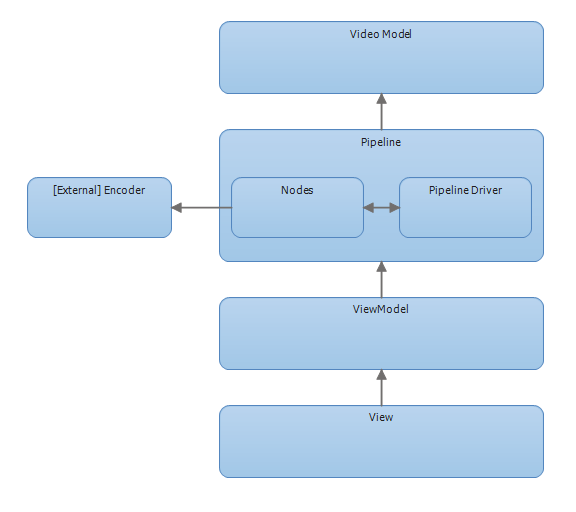
\includegraphics[scale=0.75]{resources/Layers}

\subsection{Schichtendetails}

\subsubsection*{Video Model}
Das Video Model repräsentiert ein eingelesenes Video, ggf. mit zugehörigen
Log-Daten. Da es die Daten im RGB-Format speichert, müssen diese bei Eingabe,
Ausgabe und Interaktion mit dem Encoder vom bzw. ins YUV-Format konvertiert
werden (siehe auch \hyperref[sec:produktdaten]{Produktdaten}).

\subsubsection*{Encoder}
Der zu testende Encoder ist eine externe Komponente, die nach Angabe ihres
Dateipfads vom entsprechenden Pipeline-Knoten angesprochen wird.

\newpage
\subsubsection*{Pipeline}
Die Pipeline-Schicht repräsentiert den UI-unabhängigen Aufbau des
Analyse-DAGs\footnote{\emph{directed acyclic graph}}. Sie besteht einerseits aus
den unterschiedlichen Knoten-Klassen, die unabhängig voneinander ihren
jeweiligen Algorithmus auf Frame-für-Frame-Basis implementieren, und
andererseits aus dem Pipeline Driver, der für die Abhängigkeitsauflösung und
letztendliche Abarbeitung der Pipeline zuständig ist.

\subsubsection*{ViewModel} Nach dem
Model-View-ViewModel-Pattern\footnote{\url{http://en.wikipedia.org/wiki/MVVM}}
(MVVM) ist es Aufgabe der ViewModel-Schicht, das Model der View in einer für sie
verarbeitbaren Form zu präsentieren. Bezogen auf das Projekt bedeutet dies vor
allem, die Model-Klassen um View-spezifische Daten (wie Positionierung auf der
Oberfläche) und Methoden zu ergänzen.

\subsubsection*{View}
Unter WPF wird die Oberfläche in der Beschreibungssprache
XAML\footnote{\url{http://msdn.microsoft.com/en-us/library/ms752059.aspx}}
erstellt. Sie steht über Datenbindung mit dem ViewModel in Verbindung und leitet
Benutzereingaben an dieses weiter, sodass sie selbst wenig Logik enthalten muss.

\section{Bedienoberfläche}

\setlength \fboxsep{1cm}
\begin{figure}[h!]
	\centering
    \framebox{
        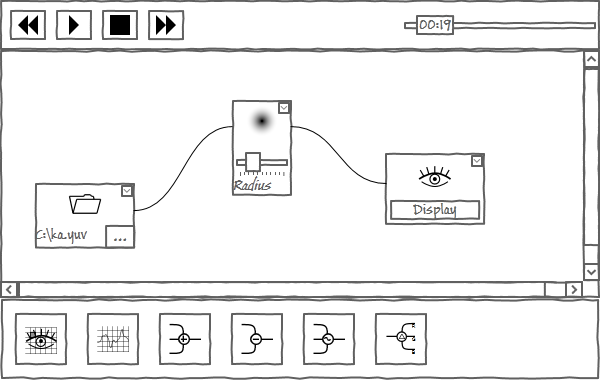
\includegraphics[scale=0.8]{resources/main-screen.png}
    }
	\caption{Hauptoberfläche des Programms}
\end{figure}
\begin{figure}[h!]
	\centering
    \framebox{
        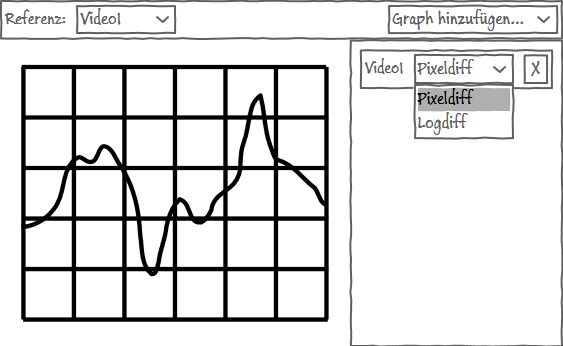
\includegraphics[scale=0.8]{resources/diagram-screen.png}
    }
	\caption{Diagrammansicht eines Outputs}
\end{figure}


\section{Qualitätszielbestimmung}

%\begin{table}[htbp]
%\begin{tabularx}{1.2\textwidth}{|l|X|X|X|X|}
\begin{tabular}{@{\extracolsep{\fill}} |l|c|c|c|c|}
\hline
Produktqualität &  Sehr gut & Gut & Normal & Nicht relevant \\ \hline
\textbf{Funktionalität} &  &  &  &  \\ \hline
Angemessenheit  &  & X &  &  \\ \hline
Richtigkeit  & X &  &  &  \\ \hline
Interoperabilität  &  &  &  & X \\ \hline
Ordnungsmäßigkeit  &  &  & X &  \\ \hline
Sicherheit  &  &  &  & X \\ \hline
\textbf{Zuverlässigkeit} &  &  &  &  \\ \hline
Reife  &  &  & X &  \\ \hline
Fehlertoleranz  &  &  & X &  \\ \hline
Wiederherstellbarkeit  &  &  & X &  \\ \hline
\textbf{Benutzbarkeit} &  &  &  &  \\ \hline
Verständlichkeit  & X &  &  &  \\ \hline
Erlernbarkeit  & X &  &  &  \\ \hline
Bedienbarkeit & X &  &  &  \\ \hline
\textbf{Effizienz} &  &  &  &  \\ \hline
Zeitverhalten  &  & X &  &  \\ \hline
Verbrauchsverhalten  &  &  & X &  \\ \hline
\textbf{Änderbarkeit} &  &  &  &  \\ \hline
Analysierbarkeit &  & X &  &  \\ \hline
Modifizierbarkeit & X &  &  &  \\ \hline
Stabilität &  & X &  &  \\ \hline
Prüfbarkeit &  & X &  &  \\ \hline
\textbf{Übertragbarkeit} &  &  &  &  \\ \hline
Anpassbarkeit &  &  &  & X \\ \hline
Installierbarkeit &  &  & X &  \\ \hline
Konformität  &  &  & X &  \\ \hline
Austauschbarkeit  &  &  &  & X \\ \hline
\end{tabular}
%\end{tabularx}
%\end{table}
%\bigskip
\paragraph{}
Es wird Wert auf die Benutzbarkeit und Modifizierbarkeit gelegt sowie auf die Angemessenheit und Richtigkeit der Funktionalität.

\section{Testfälle}

\textbf{Folgende Funktionssequenzen sind zu überprüfen:}
\begin{itemize}
	\item\textbf{/T10/} Pipeline-Konstruktion
		\begin{itemize}
			\item Der Benutzer startet das Programm.
			\item Der Benutzer wählt ``Neue Pipline erstellen''.
			\item Der Benutzer erzeugt jede Art von Knoten mindestens einmal, indem er jeden Knoten per ``Drag-and-Drop'' aus einer am unteren Bildschirmrand
				angebrachten Leiste erzeugt.
			\item Der Benutzer verbindet die erstellten Knoten miteinader, indem er Kanten zwischen den Aus- und Eingängen der Knoten erstellt.
		\end{itemize}
	\item\textbf{/T20/} Manipulation einer Pipeline
		\begin{itemize}
			\item Der Benutzer startet das Programm und erstellet eine beliebige Pipeline mit mindestens 2 Knoten, davon mindestens ein Manipulationsknoten mit Optionen 
				und mindestens einer Kante.
			\item Der Benutzer bewegt mindestens einen gesetzte Knoten innerhalb der Pipeline per ``Drag-and-Drop''.
			\item Der Benutzer verändert das Ziel mindestens einer gesetzten Kante per ``Drag-and-Drop''.
			\item Der Benutzer löscht mindestens eine Kante.
			\item Der Benutzer verändert mindestens eine Einstellung eines Manipulationsknotens.
			\item Der Benutzer löscht mindestens einen Knoten.
		\end{itemize}
	\item\textbf{/T30/} Sicherung einer Pipeline
		\begin{itemize}
			\item Der Benutzer startet das Programm und erstellet eine beliebige Pipeline.
			\item Der Benutzer speichert die Pipeline.
			\item Der Benutzer wählt ``Neue Pipeline erstellen''.
			\item Der Benutzer lädt die gesicherte Pipeline.
		\end{itemize}
\newpage
	\item\textbf{/T40/} Videoverarbeitung
		\begin{itemize}
			\item Der Benutzer startet das Programm und erstellet eine beliebige, zusammenhängende, zyklenfreie Pipeline mit mindestens einem Eingabe-, Wiedergabe- sowie 
				Manipulationsknoten mit Optionen.
			\item Der Benutzer ändert die Quelle eines Eingabeknotens.
			\item Der Benutzer öffnet den Wiedergabeknoten und beginnt das Video abzuspielen.
			\item Der Benutzer ändert mindestens eine Option eines Manipulationsknotens, während das Video abspielt.
			\item Der Benutzer ändert die Abspielgeschwindigkeit des Videos.
			\item Der Benutzer pausiert die Videowiedergabe.
			\item Der Benutzer setzt die Wiedergabe fort.
			\item Der Benutzer setzt die Videowiedergabe zurück.
			\item Der Benutzer speichert das manipulierte Video als YUV-Datei.
		\end{itemize}
	\item\textbf{/T50/} Videoanalyse
		\begin{itemize}
			\item Der Benutzer startet das Programm und erstellet eine beliebige, zusammenhängende, zyklenfreie Pipeline mit mindestens einem Eingabe-, Überlagerungs- sowie 
				Diagrammknoten.
			\item Der Benutzer deaktiviert den Diagrammknoten.
			\item Der Benutzer öffnet den Überlagerungsknoten.
			\item Der Benutzer beginnt die Videowiedergabe.
			\item Der Benutzer fügt eine Überlagerungsoption hinzu, während das Video abspielt.
			\item Der Benutzer entfernt die hinzugefügte Überlagerungsoption.
			\item Der Benutzer setzt die Videowiedergabe zurück und schließt den Überlagerungsknoten.
			\item Der Benutzer reaktiviert den Dieagrammknoten und öffnet diesen.
			\item Der Benutzer wählt ein Referenzvideo aus und fügt einen Analysegraphen hinzu.
			\item Der Benutzer startet erneut die Videowiedergabe.
			\item Der Benutzer ändert den Typ des Analysegraphen.
			\item Der Benutzer löscht den Analysegraphen.
		\end{itemize}
\end{itemize}

\newpage

\textbf{Folgende Datenkonsistenzen sind einzuhalten:}
\begin{itemize}
	\item\textbf{/T100/} Ergebnislose Wiedergabe verhindern. ~\\
		Wenn der Benutzer keinen Endknoten geöffnet hat, ist die Videowiedergabe nicht anwählbar.
	\item\textbf{/T110/} Verarbeitung ohne Eingabe verhindern. ~\\
		Falls ein Eingabeknoten ohne gültige Videoquelle mit der Pipeline verbunden ist, ist weder die Videowiedergabe, noch das Speichern von Videos als YUF-Datei möglich.
	\item\textbf{/T120/} Strukturbrüche während der Wiedergabe verhindern ~\\
		Während der Videowiedergabe kann der Benutzer die Pipelinestruktur nicht verändern.
	\item\textbf{/T130/} Inkonsistenz eines gespeicherten Videos verhindern ~\\
		Während dem Speichern eines Videos als YUF-Datei kann der Benutzer keinerlei Änderungen an der Pipeline vornehmen.
\end{itemize}

\section{Entwicklungsumgebung}

\begin{description}[style=multiline,leftmargin=4.5cm]
	\item[Betriebssystem] Windows 7
	\item[Entwicklungsumgebung] Visual Studio 2010 Ultimate + Expression Blend 4
	\item[UI-Bibliothek] WPF
	\item[Versionierung] GitHub via Git for Windows
	\item[Verfügbare Hardware] Dual- bis Hexa-Core
\end{description}

\section{Glossar}

\begin{description}
    \item[(Video-)Artefakte] Darstellungsfehler, welche sich dadurch zeigen, dass das enkodierte Video sichtlich stark von dem Referenzvideo abweicht
    \item[Asynchrone UI] Nichtblockend gestaltete Oberfläche, die bei Ladeoperationen weiterhin auf Interaktion reagiert
    \item[Differenzvideo] Videostream, welcher aus den Daten besteht, die bei der pixelweisen Subtraktion der Farbwerte zweier Videos entstehen
    \item[Drag-and-Drop] Bedienungsmuster, bei dem virtuelle Objekte mit der linken Maustaste ``gegriffen'' und ``gezogen'' werden
    \item[Farbkanal] Ein Farbbild besteht in der Regel aus 3 Farbkanälen, beispielsweise RGB (rot, grün, blau) oder \emph{YUV}.
    \item[Frame] Einzelbild eines Videos, bei \emph{H.264} unterteilt in \emph{Macroblöcke}
    \item[H.264] Weit verbreiteter \emph{Video-Codec} und Ziel-Codec der zu testenden Encoder
    \item[Histogramm] Diagrammart ähnlich einem Balkendiagramm, welche aber auch den Flächeninhalt eines Balken korrekt skaliert darstellt
    \item[Interface, UI] Benutzeroberfläche. Man unterscheidet zwischen Konsolenoberfläche und graphischer Oberfläche.
    \item[Inter-Frame] Videoframe, dessen Daten aus einem oder mehreren benachbarten Frames berechnet werden
    \item[Intra-Frame] Videoframe, dessen Daten unabhängig von denen anderer Frames gespeichert sind. Vergleiche \emph{Inter-Frame}.
    \item[Macroblock] Bei \emph{H.264} 16x16 Pixel große Blöcke, in die jeder \emph{Frame} aufgeteilt wird. Im Gegensatz zu älteren Codecs kann bei H.264 für jeden Macroblock eine unterschiedliche \emph{Inter/Intra-Frame}-Entscheidung getroffen werden. 
    \item[Move Vector] Vektor, um den jeder Referenzframe eines \emph{Inter-Frames} zusätzlich verschoben werden kann. Ermöglicht eine effiziente Kodierung von verschiebenden Bewegungen.
    \item[Multithreading] Programmiertechnik, in der die zu verrichtende Arbeit auf mehrere Prozessfäden verteilt wird. Dies ermöglicht Parallelismus und die optimale Auslastung von Multikern-Systemen
    \item[Noise] Ein randomisiertes Signal. Allgemein als ``Bildrauschen'' zu verstehen.
    \item[Overlay] Ein transparent über ein anderes Objekt gezeichnetes Objekt
    \item[Peak signal-to-noise ratio] Maß für den wahrgenommenen Qualitätsverlust eines komprimierten Videoframes
    \item[Pipeline] Hintereinanderschaltung von verschiedenen Knotentypen zum Einlesen, Modifizieren und Analysieren von Videos, in der UI dargestellt als Graph mit über \emph{Drag-and-Drop} erstellbaren Kanten
    \item[Resolution] Bildauflösung
    \item[Undo/Redo] ``Aktion zurücknehmen/wiederholen''
    \item[Video-Codec] Spezifikation eines Verfahrens, um Videodaten (meist verlustbehaftet) zu komprimieren
    \item[Videoencoder] Programm, welches rohe Videodaten als Eingabe annimmt und in einem bestimmten \emph{Video-Codec} entsprechendes Format bringt
    \item[YUV] Eine Familie von Farbpaletten, welche die Sehart des menschlichen Auges in Betracht nehmen
\end{description}



\end{document}
